\PassOptionsToPackage{unicode}{hyperref}
\documentclass[aspectratio=1610, professionalfonts, 9pt]{beamer}

\usefonttheme[onlymath]{serif}
\usetheme[showtotalframes]{tudo}

\ifluatex
\usepackage{polyglossia}
\setmainlanguage{german}
\else
\ifxetex
\usepackage{polyglossia}
\setmainlanguage{german}
\else
\usepackage[german]{babel}
\fi
\fi


% Mathematik
\usepackage{amsmath}
\usepackage{amssymb}
\usepackage{mathtools}
\usepackage{cancel}

\usepackage{hyperref}
\usepackage{bookmark}

% Bibliographie 
\usepackage[
  backend=biber,   
  autolang=hyphen,
  citestyle=verbose, 
  giveninits=true,
]{biblatex}
\addbibresource{references.bib} 
\DefineBibliographyStrings{german}{andothers = {{et\,al\adddot}}}

%%%%%%%%%%%%%%%%%%%%%%%%%%%%%%%%%%%%%%%%%%%%%%%%%%%%%%%%%%%%%%%%%%%%%%%%%%%%%%%%
%%%%%-------------Hier Titel/Autor/Grafik/Lehrstuhl eintragen--------------%%%%%
%%%%%%%%%%%%%%%%%%%%%%%%%%%%%%%%%%%%%%%%%%%%%%%%%%%%%%%%%%%%%%%%%%%%%%%%%%%%%%%%

%Titel:
\title{Gamma/Hadron-Seperation bei FACT}
%Autor
\author[M.~Sackel]{Maximilian Sackel}
%Lehrstuhl/Fakultät
\institute[Experimental Physics 5]{Experimental Physiks 5b \\  Astroteilchenphysik}
%Titelgrafik 
\titlegraphic{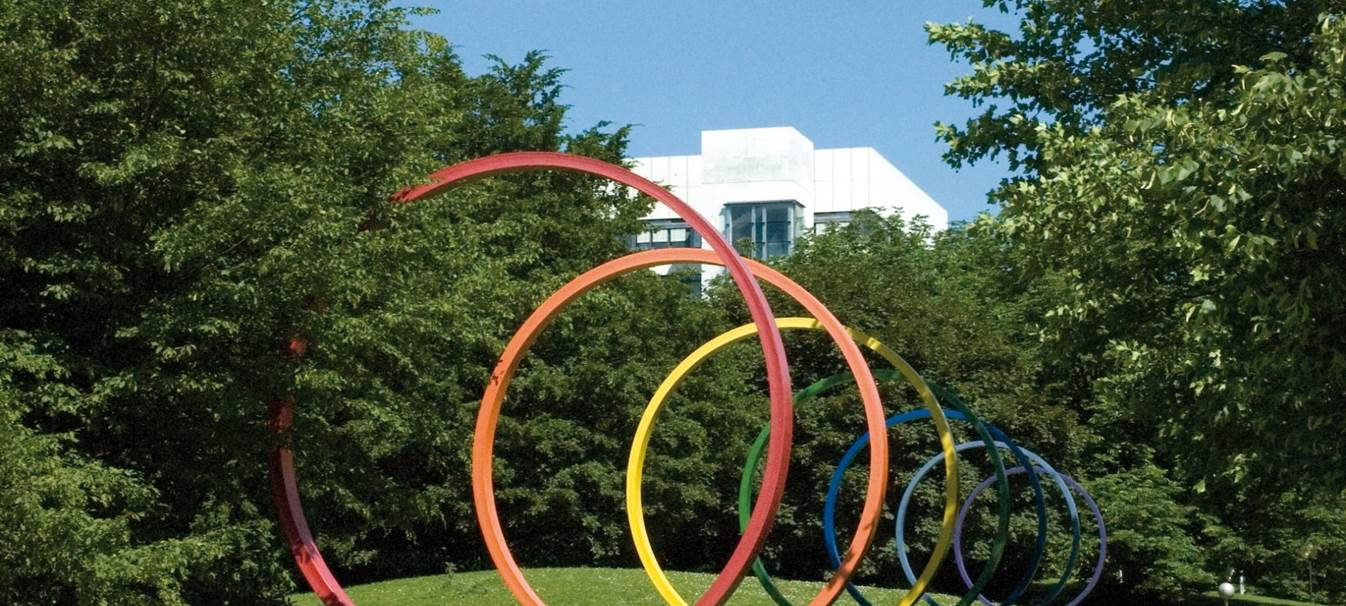
\includegraphics[width=0.7\textwidth]{images/tudo-title-2.jpg}}


\begin{document}

\maketitle

\begin{frame}
  \begin{figure}
	\centering
	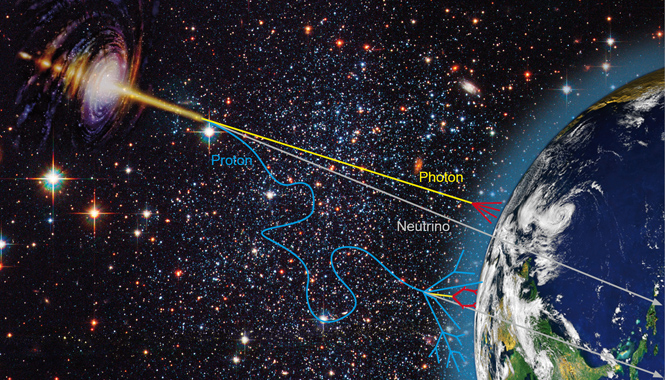
\includegraphics[width=0.8\textwidth]{./images/sources-detection.jpg} \\
	\caption{\cite{Overview}}
  \end{figure}
\end{frame}

\begin{frame}
  \begin{columns}
	\column{.3\textwidth}
	\begin{figure}
	  \centering
	  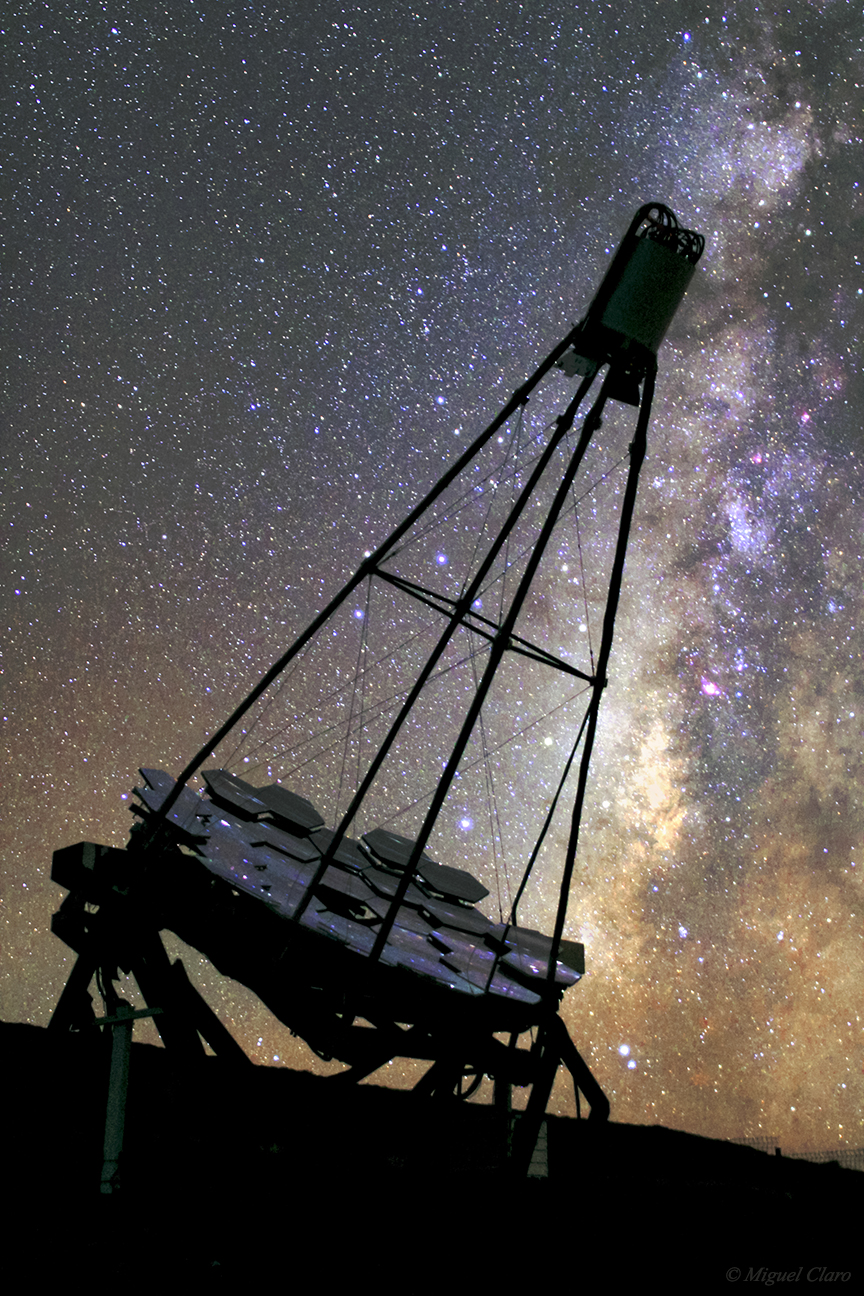
\includegraphics[height=0.8\textheight]{./images/FACT.jpg}
	  \caption{\cite{FACT}}
	\end{figure}
	\column{.7\textwidth}
	\only<1>{
	\Huge
	\centering
	\textbf{F}irst G-\textbf{A}PD \textbf{C}herenkov \textbf{T}elescope
  	}
	\only<2>{
	  \begin{figure}
		\centering
		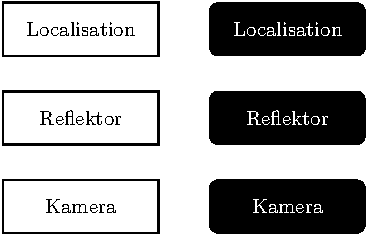
\includegraphics[height=0.8\textheight]{./tikz/FACT/FACT.pdf}
	  \end{figure}
	}
  \end{columns}
\end{frame}

\begin{frame}
  \begin{columns}
	\column{.2\textwidth}
	\begin{figure}
	  \centering
	  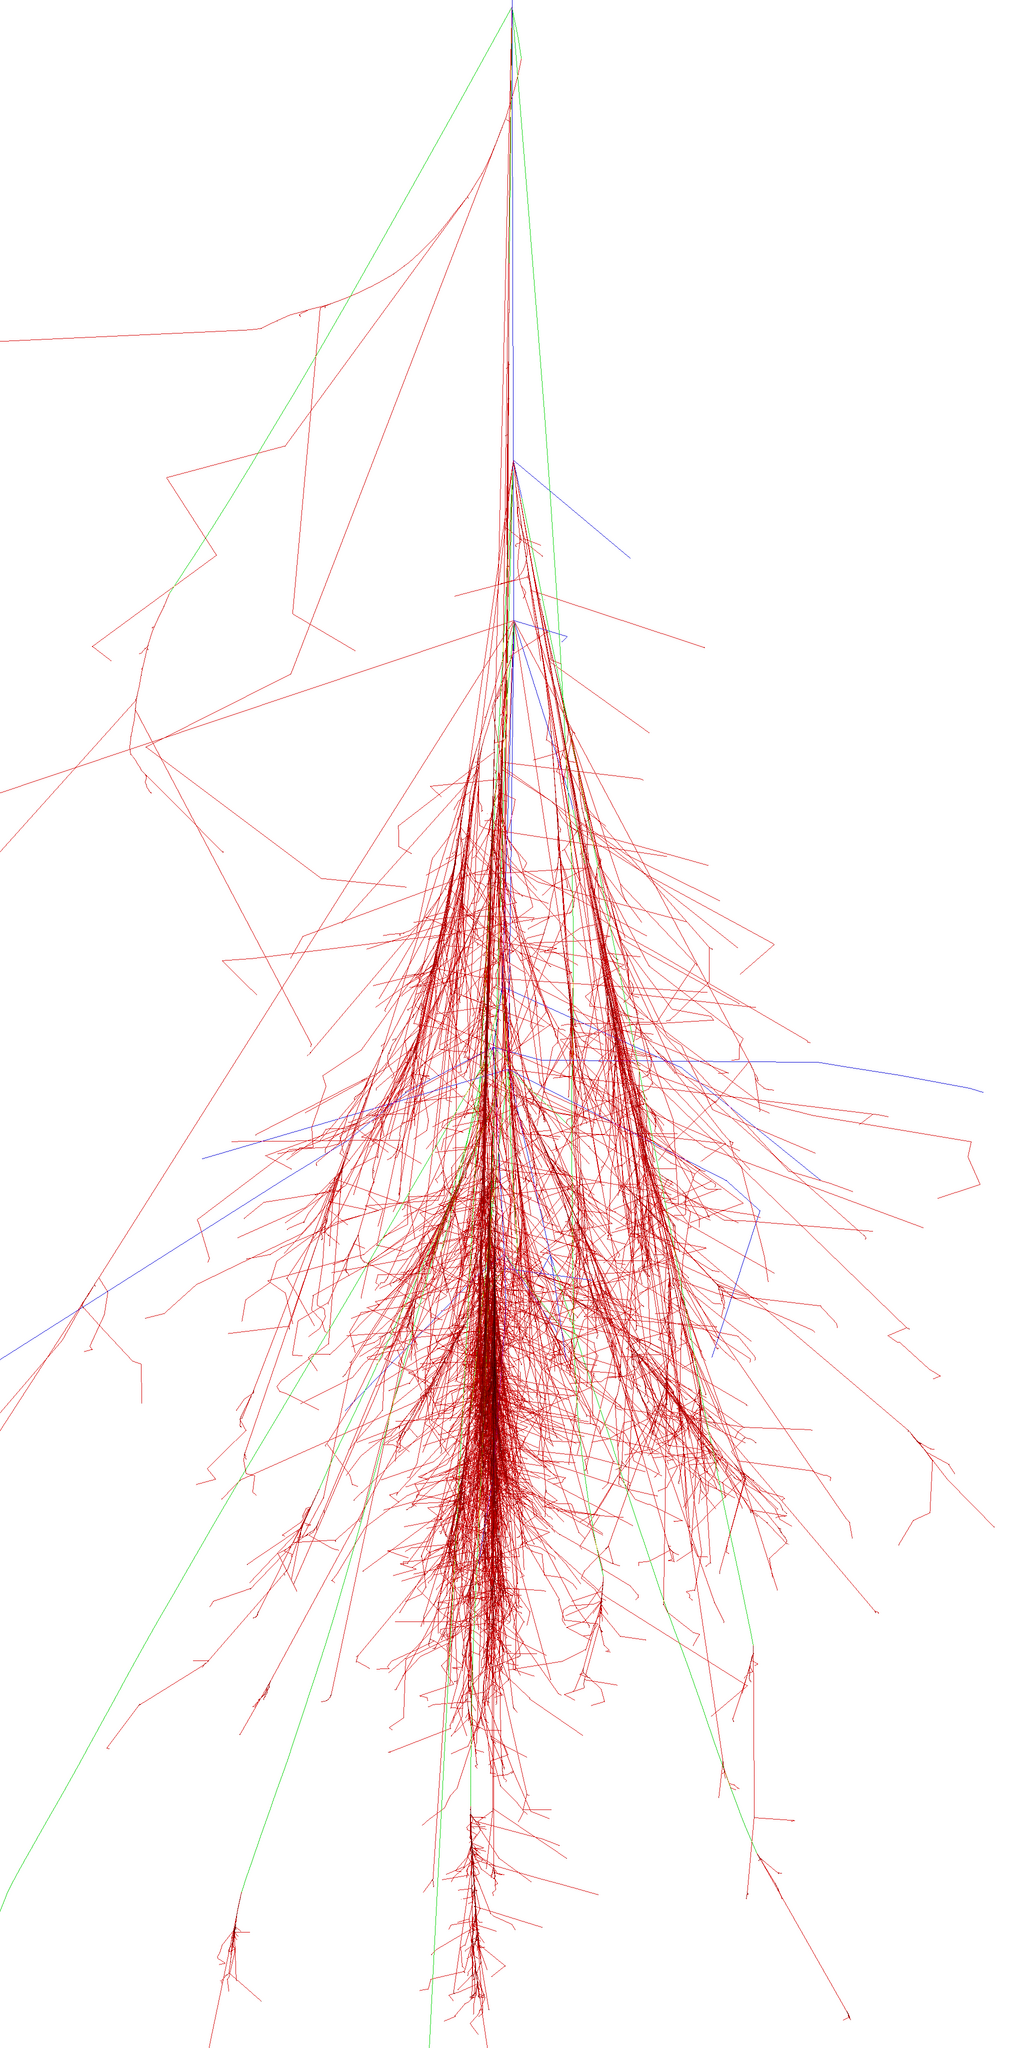
\includegraphics[width=\textwidth]{./images/proton_100GeV.png}
	  \caption{\cite{FACT}}
	\end{figure}
	\column{.3\textwidth}
	\begin{eqnarray*}
	  \pi^{0} \rightarrow& \gamma + \gamma \\
	  \pi^{+} \rightarrow& \mu^{+} + \nu_{\mu} \\
	  \pi^{-} \rightarrow& \mu^{-} + \bar{\nu}_{\mu}
	\end{eqnarray*}
	\column{.2\textwidth}
	\begin{figure}
	  \centering
	  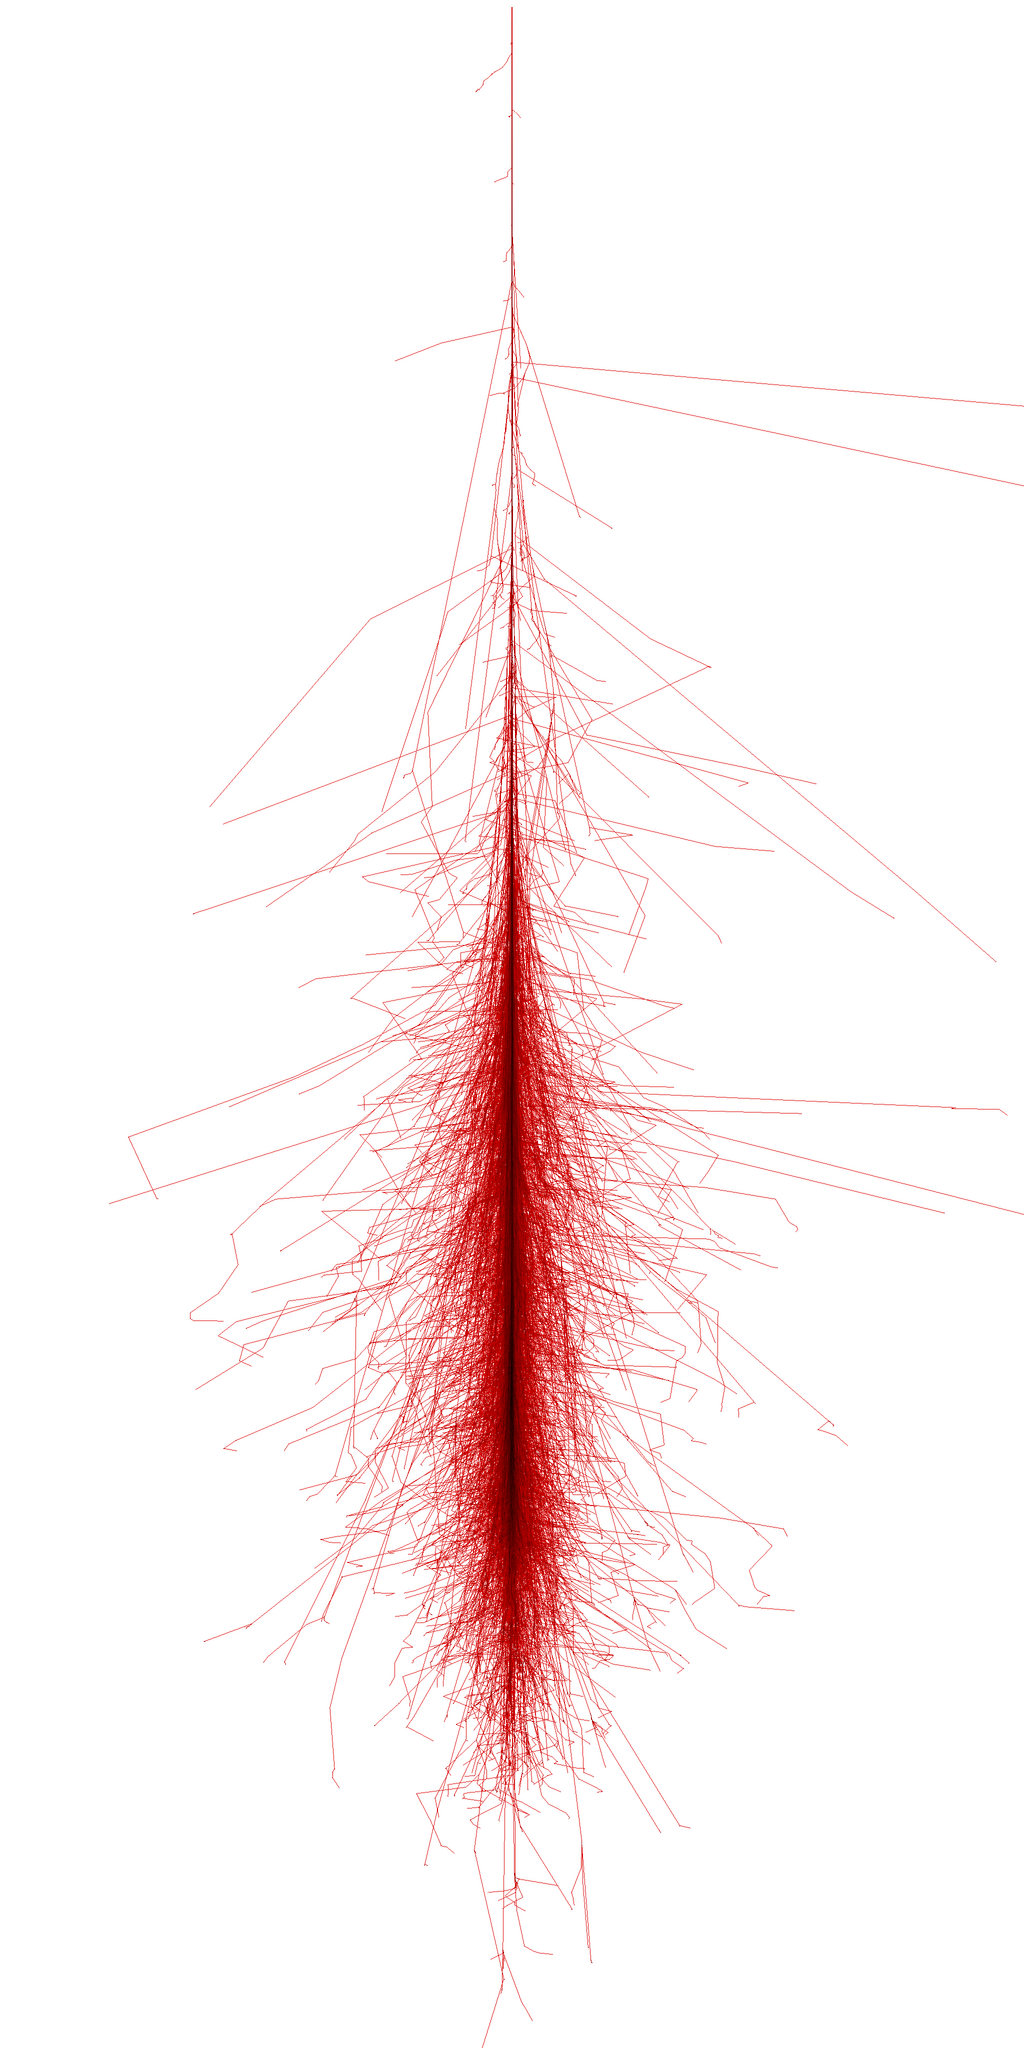
\includegraphics[width=\textwidth]{./images/photon_100GeV.png}
	  \caption{\cite{FACT}}
	\end{figure}
	\column{.3\textwidth}
	\begin{eqnarray*}
	  \gamma \rightarrow& e^{+} + e^{-} \\
	  e^{+} \rightarrow& e^{+'} + \gamma \\
	  e^{-} \rightarrow& e^{-'} + \gamma 
	\end{eqnarray*}
  \end{columns}
\end{frame}

\begin{frame}
  \begin{columns}
	\column{.5\textwidth}
	\begin{figure}
	  \centering
	  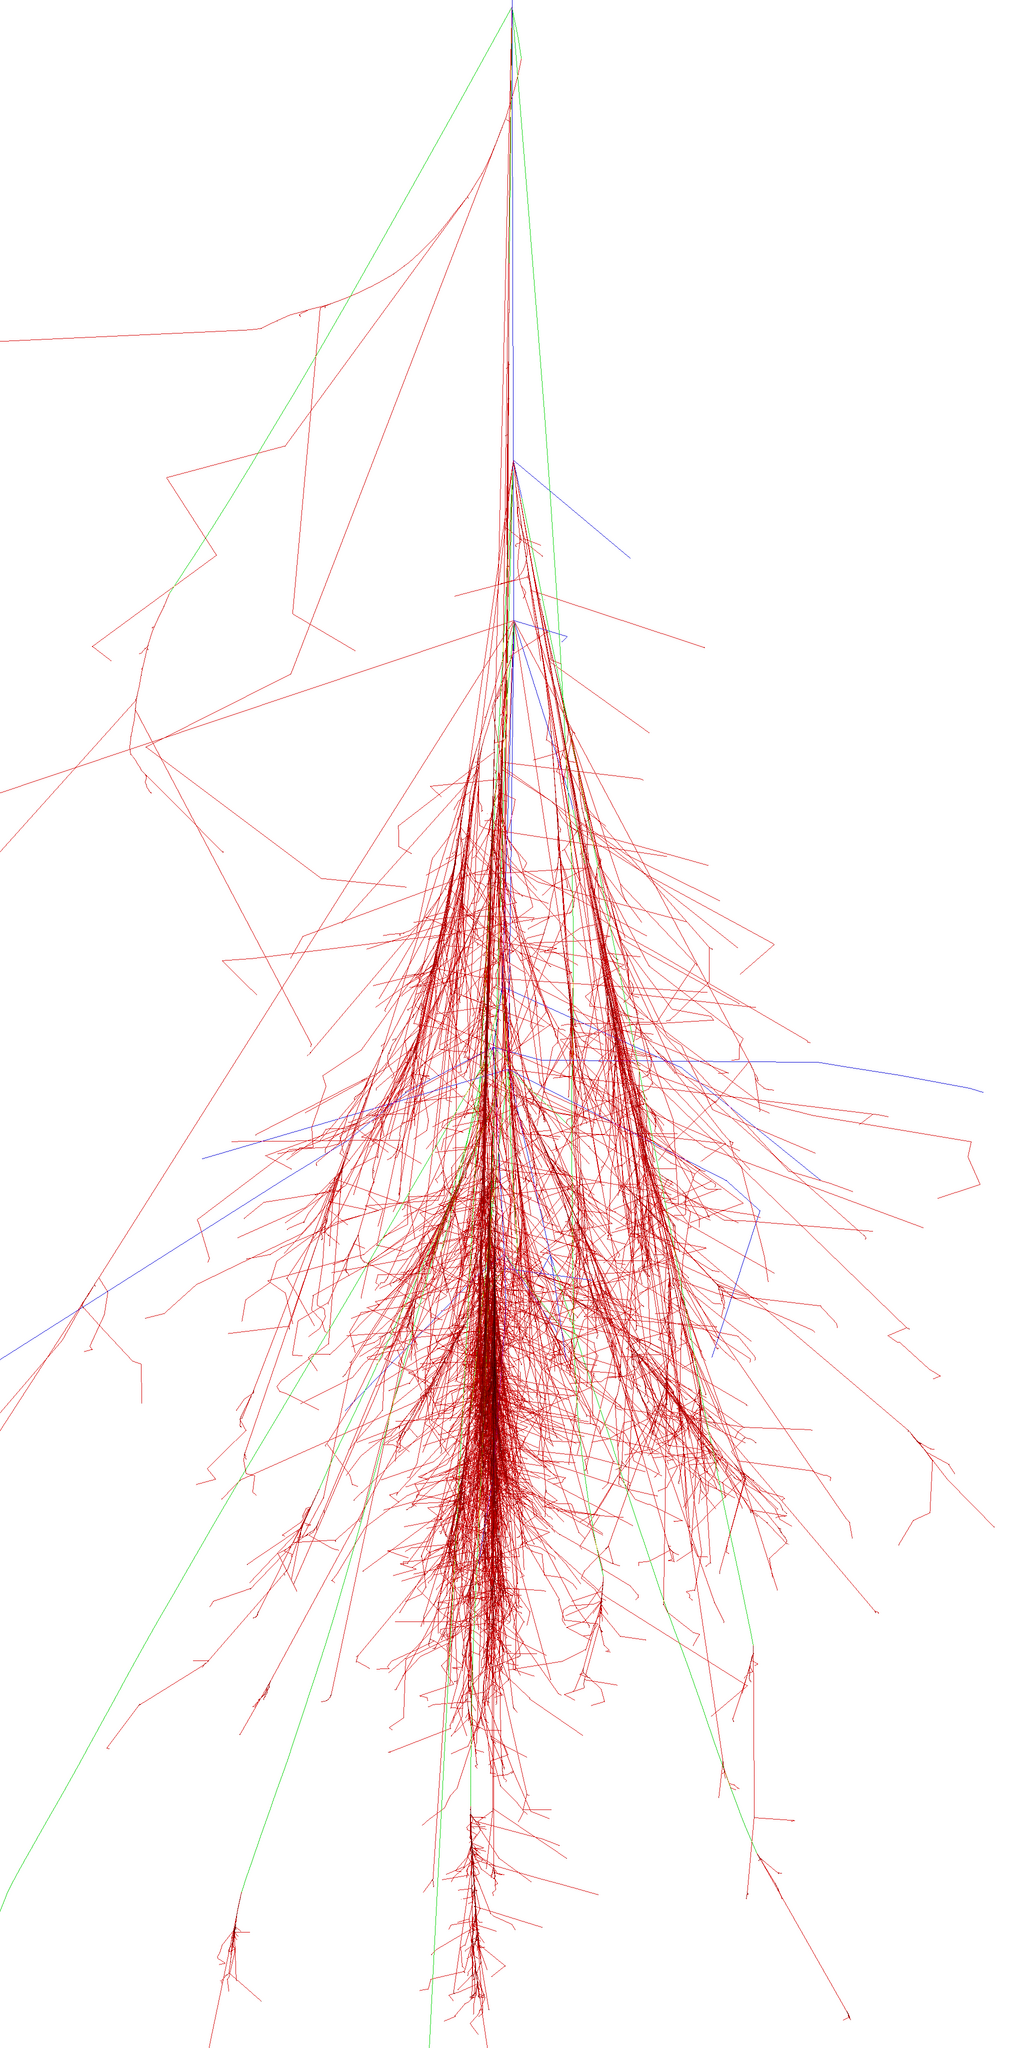
\includegraphics[width=\textwidth]{./images/proton_100GeV.png}
	  \caption{\cite{FACT}}
	\end{figure}
	\column{.5\textwidth}
	\begin{figure}
	  \centering
	  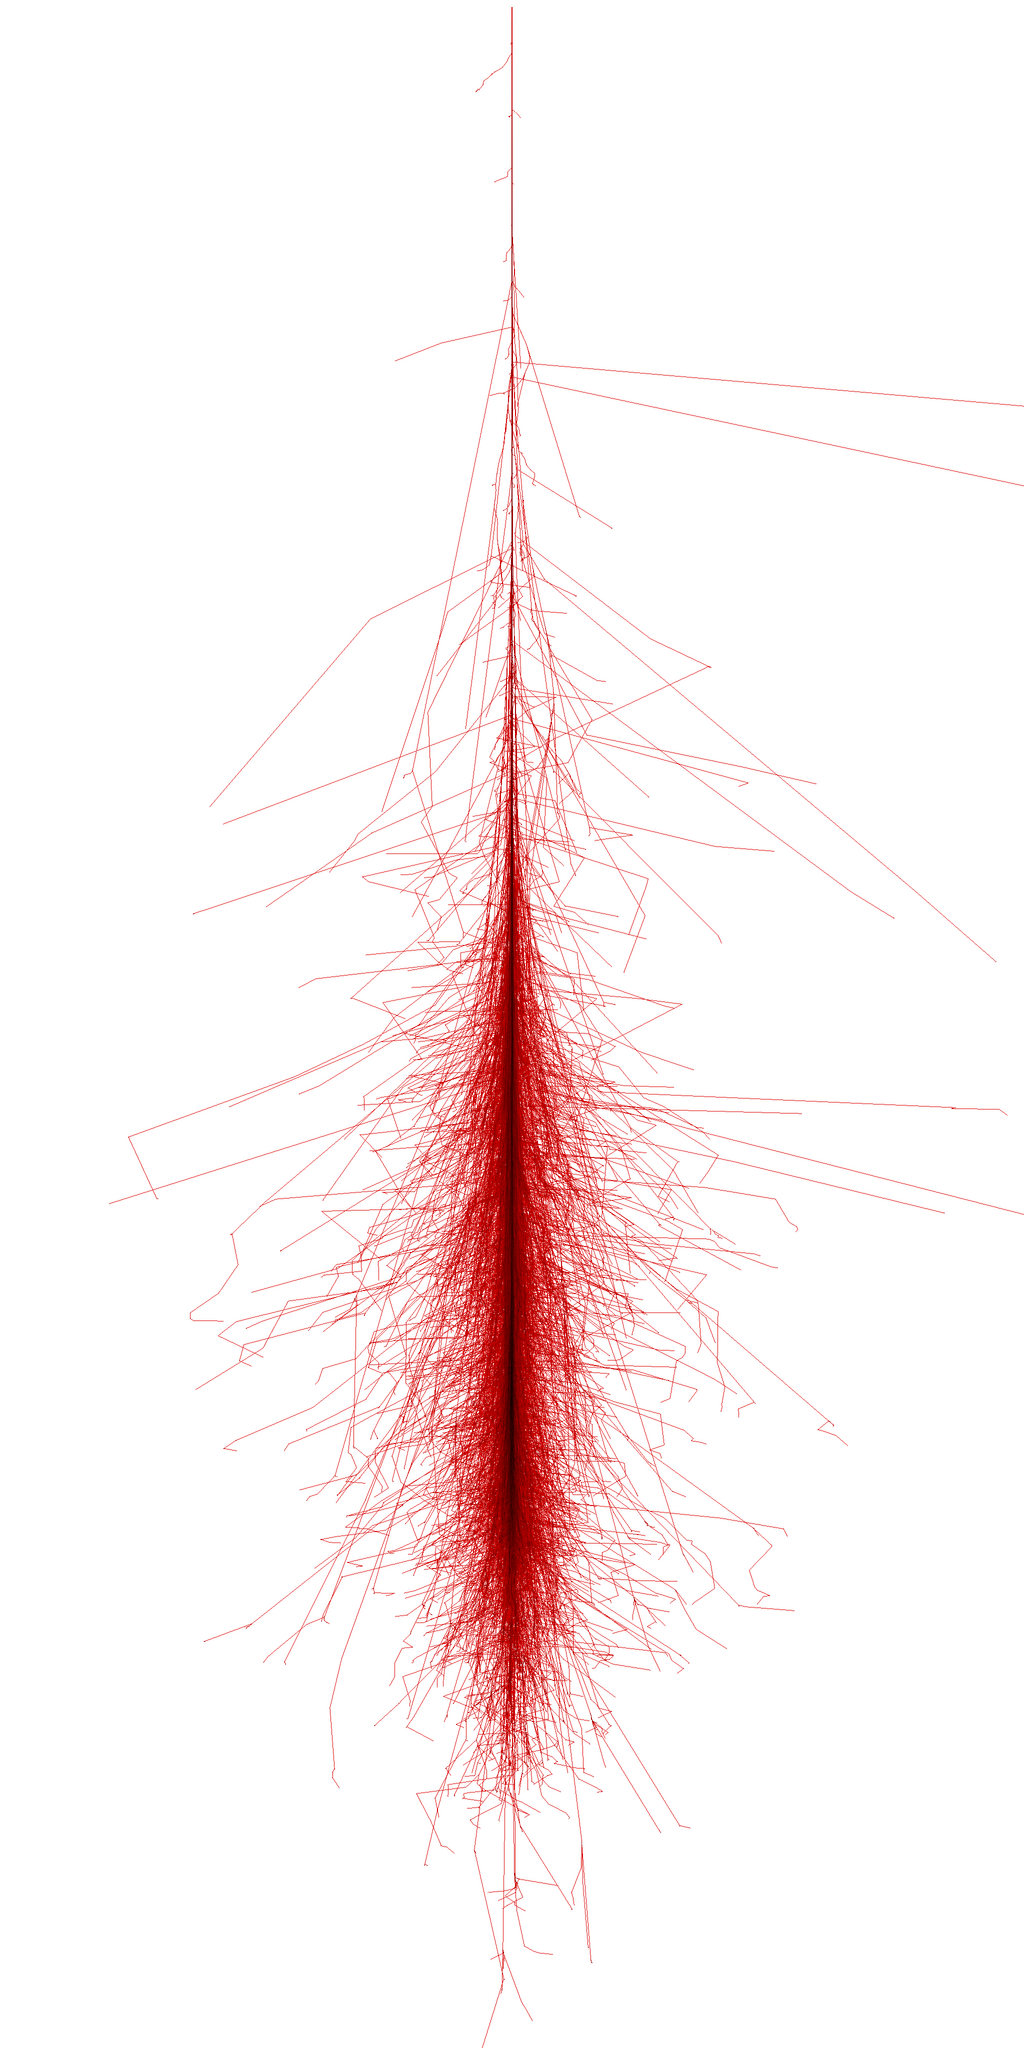
\includegraphics[width=\textwidth]{./images/photon_100GeV.png}
	  \caption{\cite{FACT}}
	\end{figure}
  \end{columns}
\end{frame}
\section{Blindtext}
\begin{frame}
  \frametitle{Hier steht eine lange, zweizeilige Headline
  \newline gefolgt von einem Blindtext}
  Dieser Text dient nur zur Veranschaulichung des Textsatzes. Niemand sollte jemals, aus keinem noch so gutem Grund, so viel Text auf eine Folie packen.

  Dies ist ein Blindtext. Dieser Text ist nicht dafür vorgesehen, den Betrachter in die Welt der Dunkelheit zu führen, sondern dafür, einfach etwas Leeres mit etwas Inhaltlosem zu füllen.

  Dies ist ein Blindtext. Dieser Text ist nicht dafür vorgesehen, den Betrachter in die Welt der Dunkelheit zu führen, sondern dafür, einfach etwas Leeres mit etwas Inhaltlosem zu füllen.

  Dies ist ein Blindtext. Dieser Text ist nicht dafür vorgesehen, den Betrachter in die Welt der Dunkelheit zu führen, sondern dafür, einfach etwas Leeres mit etwas Inhaltlosem zu füllen.
\end{frame}

\begin{frame}{title}
  \begin{enumerate}
	\item test
	\item test
  \end{enumerate}
\end{frame}

\begin{frame}{title}
  \begin{block}{title}
	ANlsnldas dkmadföonslkadm x
  \end{block}
\end{frame}
\end{document}
